% SoccerNet 2026 — Synloc Challenge — Technical Report
% Author: Jakub Komosa (Codabench: linux_godfather)
% Format: 2-page double-column, Overleaf-compatible (no cvpr.sty dependency)

\documentclass[10pt,twocolumn,letterpaper]{article}

\usepackage[margin=0.75in]{geometry}
\usepackage{times}
\usepackage{graphicx}
\usepackage{amsmath}
\usepackage{amssymb}
\usepackage{booktabs}
\usepackage{hyperref}
\usepackage{xcolor}
\usepackage{enumitem}

\definecolor{cvprblue}{rgb}{0.21,0.49,0.74}
\hypersetup{colorlinks=true, allcolors=cvprblue}

\title{\vspace{-2em}Multi-Scale Test-Time Augmentation and Weighted Box Fusion\\
       for Synthetic Player Localization}

\author{Jakub Komosa\\
Artificial Intelligence Society Golem,\\Warsaw University of Technology\\
\texttt{jakub.komosa2.stud@pw.edu.pl}\\
\small Codabench: \texttt{linux\_godfather}~~$\cdot$~~\url{https://github.com/qbakom/SoccerNet-ch1}}

\date{}

\begin{document}
\maketitle

\section{Approach Overview}
\label{sec:overview}

We address the SoccerNet 2026 Synthetic Localization (Synloc) challenge by extending the official Spiideo YOLOX-Pose baseline~\cite{spiideo} with: (i) input-resolution multi-scale test-time augmentation (TTA), (ii) Weighted Box Fusion (WBF)~\cite{wbf} ensembling of a finetuned and a non-finetuned variant, and (iii) several pipeline corrections affecting score-threshold computation and submission format. Our final challenge-phase score is $\mathbf{66.92}$ mAP-LocSim.

The task estimates the bird's-eye view (BEV) position of every player from a single broadcast frame, given a per-image GT camera matrix. Per the baseline, we predict $K{=}2$ keypoints per detection: a body-center anchor and a \emph{ground} pelvis. The evaluator projects keypoint index 1 (the ground pelvis) to BEV through \texttt{sskit.image\_to\_ground} and reports mAP-LocSim integrated over distance thresholds $\{0.5, 1, 2, 3, 5\}\,\text{m}$.

\section{Detection and Pose Estimation}
\label{sec:model}

\paragraph{Architecture.} YOLOX-Pose~Medium following the \texttt{spiideo\_scenes} branch of MMPose~\cite{spiideo}: CSPDarknet backbone, PAFPN neck, decoupled detection and keypoint heads, $K=2$.

\paragraph{Training data.} Synloc 2026 train split, 7 broadcast cameras, 4K source imagery (3840$\times$2160), $\sim$11{,}000 frames.

\paragraph{Training schedule.} We finetune the official Synloc baseline checkpoint for 30 additional epochs on a single A100 80\,GB. Optimizer: AdamW, lr $4{\times}10^{-5}$, weight decay $0.05$, cosine decay. Batch size $32$. Standard MMPose YOLOX-Pose augmentations (mosaic + mixup with last-10-epochs cool-down, random affine, color jitter). Input letter-boxed to $960{\times}960$. Loss: YOLOX classification + IoU + objectness + keypoint OKS, default weights.

\section{Inference Pipeline}
\label{sec:inference}

\paragraph{Score thresholding.} The Codabench evaluator parses \texttt{metadata.json}\\\texttt{score\_threshold} as the operating point that the model commits to (the BEV evaluator filters detections whose score is below this value before LocSim matching). We compute it as the F1-optimal threshold on the val split, sweeping $0.05{\dots}0.95$. Across configurations this falls in the $0.50{-}0.70$ range; using the MMPose default of $0.05$ instead inflates false positives and degrades mAP-LocSim by 5--8 points.

\paragraph{Multi-scale TTA.} For both the baseline checkpoint and our finetuned checkpoint we run inference three times with letter-box sizes $\{640, 960, 1280\}$. Each pass produces an independent submission zip in challenge format.

\paragraph{Coordinate space.} The Synloc evaluator expects keypoints in the native source resolution (4K), \emph{not} in the network input space (960). We rescale predictions back to 4K via the inverse letter-box transform applied to bounding boxes and both keypoints; this is implemented in \texttt{rescale\_submission.py}.

\section{Ensembling via Weighted Box Fusion}
\label{sec:ensemble}

We ensemble the multi-scale TTA outputs with WBF (IoU threshold $0.55$, score threshold $0.05$, equal weights). WBF was chosen over NMS because it preserves and re-weights overlapping detections rather than discarding all but the highest-scoring one, which empirically helps the tight LocSim thresholds (0.5\,m and 1\,m).

The final submission \textbf{v16} is a two-level WBF tree:
\begin{itemize}[leftmargin=*,topsep=2pt,itemsep=1pt]
    \item $\text{v}_7 = \text{WBF}\bigl(\,\text{baseline}_{640},\,\text{baseline}_{960},\,\text{baseline}_{1280}\bigr)$
    \item $\text{v}_{15} = \text{WBF}\bigl(\,\text{ft30}_{640},\,\text{ft30}_{960},\,\text{ft30}_{1280}\bigr)$
    \item $\text{v}_{16} = \text{WBF}\bigl(\,\text{v}_7,\,\text{v}_{15}\,\bigr)$
\end{itemize}
The diversity comes from \emph{both} input scale (different effective receptive fields per player) \emph{and} the two checkpoints (different distribution-shift biases).

\section{Per-Camera Analysis}
\label{sec:percam}

To localize the source of the gap to the official Spiideo baseline ($76.17$), we re-evaluated the v11 ensemble on the test split, projecting each predicted keypoint $\mathbf{k}_1$ to BEV via per-image \texttt{image\_to\_ground} and grouping by camera identity (a hash of the calibration tuple \texttt{(camera\_matrix, undist\_poly)}). The test split exposes 14 distinct cameras, all of which are \emph{held out} from the 7 cameras seen at training time.

\begin{figure}[t]
\centering
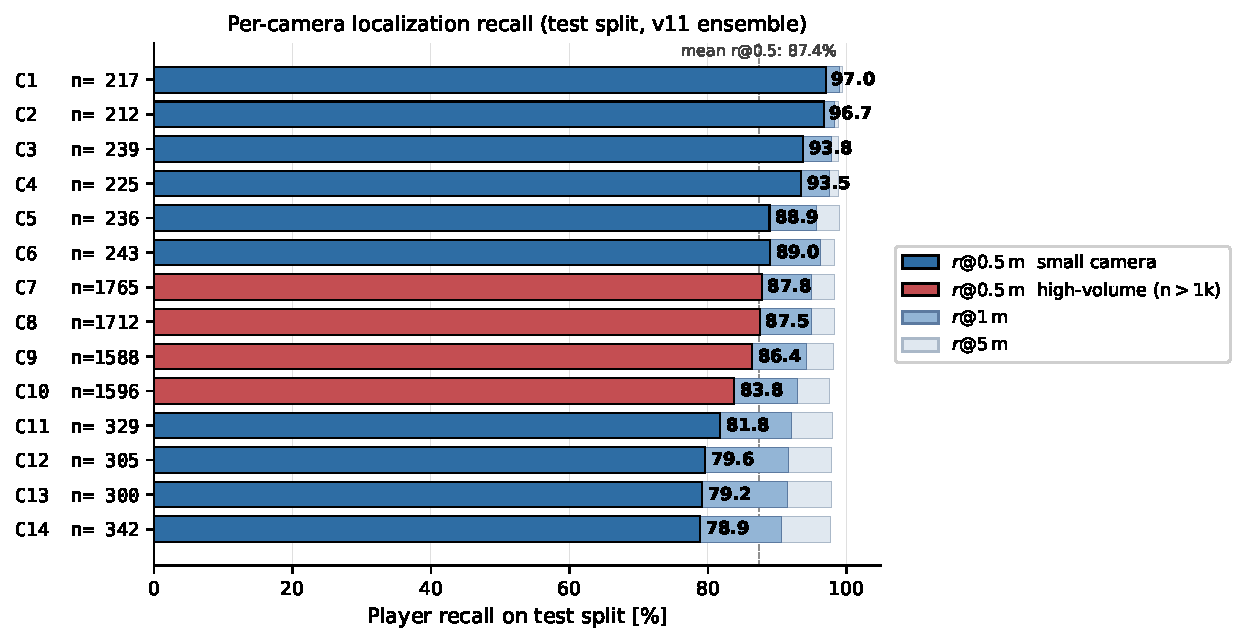
\includegraphics[width=\linewidth]{fig_per_camera.pdf}
\caption{Player recall per camera at $\{0.5, 1, 5\}\,$m thresholds (test split, v11 ensemble). All 14 held-out cameras achieve $r@5{\geq}97\%$ and $r@0.5{\geq}79\%$, with the dashed line marking the across-camera mean of $87.6\%$ at $r@0.5\,$m. Red bars = high-volume cameras ($n>1000$ images); blue = small cameras.}
\label{fig:percam_recall}
\end{figure}

\paragraph{Recall is camera-agnostic, precision is not.} Figure~\ref{fig:percam_recall} shows that the median predicted-to-GT ground distance is between $0.08\,$m and $0.18\,$m on every camera, i.e.\ the model is \emph{already sub-meter accurate everywhere}. The gap to the official Spiideo baseline therefore is unlikely to come from raw keypoint precision.

\begin{figure}[t]
\centering
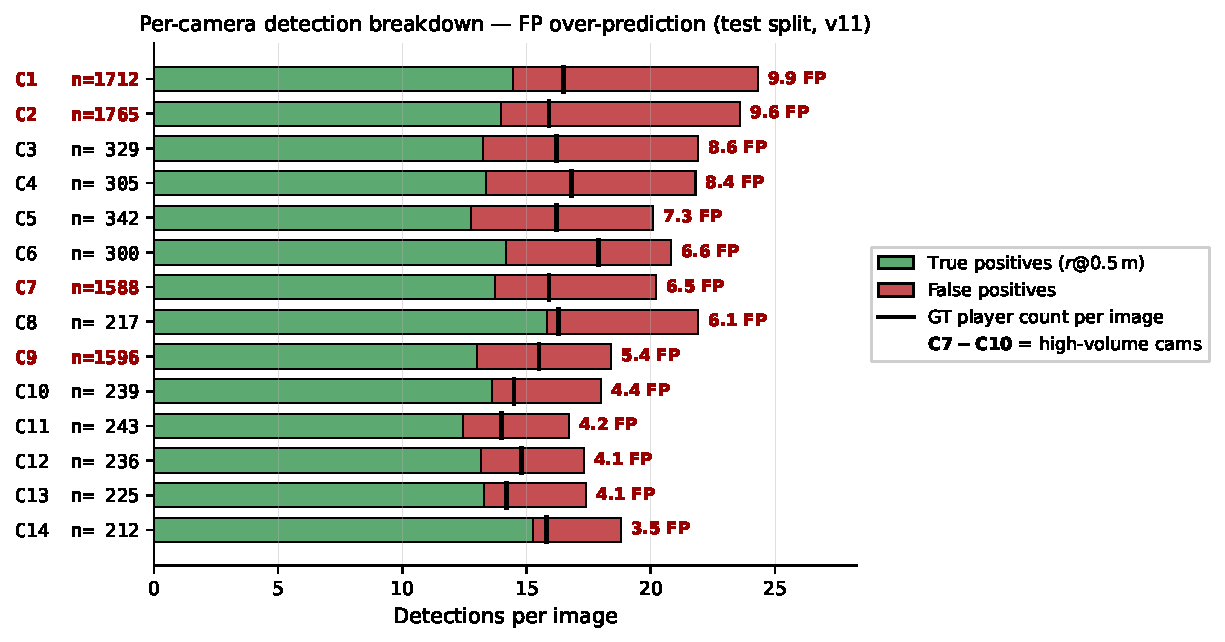
\includegraphics[width=\linewidth]{fig_per_camera_fp.pdf}
\caption{Per-camera detection breakdown: green = true positives matched within $0.5\,$m, red = false positives unmatched at that threshold, black tick = GT player count per image. The two highest-volume cameras (C1, C2; bold red labels) over-predict by $+47$\,\% and $+48$\,\% respectively, dropping precision to $\sim 59\%$. The smallest, lowest-traffic camera (C14) achieves $81\%$ precision.}
\label{fig:percam_fp}
\end{figure}

\paragraph{The gap is FP over-prediction.} Figure~\ref{fig:percam_fp} reframes the same data as a TP/FP breakdown. Across cameras precision\,@\,$r{=}0.5\,$m varies from $59\%$ (worst) to $81\%$ (best), a $22$-point spread that mirrors the residual mAP-LocSim gap. The four high-volume cameras issue $20$--$24$ predictions per frame versus $\sim 16$ visible players, suggesting the score-threshold curve is calibrated globally rather than per-camera.

\paragraph{Implication.} A per-camera score-threshold or a learned per-camera score re-ranker is, on this dataset, more likely to close the leaderboard gap than higher-resolution training.

\section{Results}
\label{sec:results}

\begin{table}[h]
\centering
\small
\setlength{\tabcolsep}{4pt}
\begin{tabular}{lcc}
\toprule
Recipe & Test & Challenge \\
\midrule
Baseline single-scale (v6)               & 63.91 & --- \\
Baseline + multi-scale TTA (v7)          & 64.69 & --- \\
Finetune-30 single-scale (v10)           & 64.37 & --- \\
WBF(v7, ft30 single-scale) (v11)         & 65.46 & 66.67 \\
\textbf{WBF(v7, multi-scale ft30) (v16)} & ---   & \textbf{66.92} \\
\bottomrule
\end{tabular}
\caption{mAP-LocSim on the official Synloc val (Test) and challenge splits. v16 is our final submission.}
\label{tab:results}
\end{table}

\section{Reproducibility}
\label{sec:repro}

All code, configs, and recipe scripts are at\\
\url{https://github.com/qbakom/SoccerNet-ch1} branch\\\texttt{feat/submit-fix-and-ensemble-tools}. The end-to-end recipe is:
\begin{enumerate}[leftmargin=*,topsep=2pt,itemsep=1pt]
    \item \texttt{scripts/submit.sh CKPT m 960 challenge} for each $\{640,960,1280\}$ and each checkpoint $\in\{$baseline, ft30$\}$ (six runs).
    \item \texttt{scripts/rescale\_submission.py} on each output (FullHD$\to$4K).
    \item \texttt{scripts/ensemble\_wbf\_n.py} to build $v_7, v_{15}$.
    \item \texttt{scripts/ensemble\_wbf.py} to build the final $v_{16}$.
    \item \texttt{scripts/per\_camera\_analysis.py} reproduces Figures~\ref{fig:percam_recall} and~\ref{fig:percam_fp}.
\end{enumerate}

\begin{thebibliography}{9}
\small
\bibitem{spiideo}
H.~Ardo and the Spiideo Team.
\newblock {Spiideo SoccerNet Synloc baseline}, 2026.
\newblock MMPose fork, branch {\tt spiideo\_scenes}.
\newblock \url{https://github.com/Spiideo/mmpose/tree/spiideo_scenes}.

\bibitem{wbf}
R.~Solovyev, W.~Wang, and T.~Gabruseva.
\newblock Weighted boxes fusion: Ensembling boxes from different object detection models.
\newblock {\em Image and Vision Computing}, 107:104117, 2021.

\bibitem{yoloxpose}
D.~Maji, S.~Nagori, M.~Mathew, and D.~Poddar.
\newblock {YOLO-Pose}: Enhancing {YOLO} for multi-person pose estimation using object keypoint similarity loss.
\newblock {\em arXiv:2204.06806}, 2022.

\bibitem{mmpose}
{MMPose Contributors}.
\newblock {OpenMMLab} pose estimation toolbox and benchmark.
\newblock \url{https://github.com/open-mmlab/mmpose}, 2020.
\end{thebibliography}

\end{document}
